\chapter{TINJAUAN PUSTAKA}

\section{Hasil Penelitian Terdahulu}
Penelitian mengenai translasi isometri matematika geometri klasik ke geometri tropikal dan pelipatan tegar telah dibahas pada berbagai literatur. Ringkasan sintesis hasil penelitian terdahulu yang mendasari dan memotivasi riset tesis ini disajikan pada \ref{tab:penelitian_terdahulu}.

\bgroup
\renewcommand{\arraystretch}{1.5}
\begin{longtable}{|c|p{3.2cm}|c|p{8.5cm}|}
  \caption{Matriks Hasil Penelitian Terdahulu}
  \label{tab:penelitian_terdahulu} \\
  \hline
  \textbf{No} & \textbf{Peneliti}                  & \textbf{Tahun}                   & \textbf{Fokus \& Kontribusi Penelitian} \\
  \hline
  \endfirsthead
  
  \multicolumn{4}{c}%
  {{\thetable{} -- Lanjutan dari halaman sebelumnya}} \\
  \hline
  \textbf{No} & \textbf{Peneliti}                  & \textbf{Tahun}                   & \textbf{Fokus \& Kontribusi Penelitian} \\
  \hline
  \endhead
  
  \hline
  \endfoot
  
  \hline
  \endlastfoot

  % Tabel sengaja dikosongkan — akan diisi setelah literature review baru selesai.
  
\end{longtable}
\egroup

\section{Origami Matematis}
Matematika origami mempelajari batasan geometris dan kombinatoris dari selembar kertas yang dilipat tanpa disobek atau diregangkan. Pada pelipatan datar (\textit{flat folding}), keseluruhan kertas pada akhirnya dapat ditekan hingga rata di atas bidang dua dimensi \parencite{hull2012project}.

\subsection{Pola Lipatan}
Proses melipat kertas dapat diabstraksikan menjadi sebuah graf yang menempel pada selembar kertas datar. Graf ini memetakan jejak lipatan yang ditinggalkan saat kertas dibuka kembali.
\begin{definisi}
  Sebuah pola lipatan (\textit{crease pattern}) adalah sebuah graf planar yang diletakkan pada suatu daerah $D \subset \R^2$. Verteks dari graf tersebut disebut sebagai verteks origami, dan sisi (edge) dari graf tersebut disebut sebagai garis lipatan (\textit{creases}).
\end{definisi}

\begin{contoh}
  Perhatikan sebuah verteks tunggal $v$ yang terletak di interior selembar kertas persegi, dengan empat garis lipatan $l_1, l_2, l_3, l_4$ memancar dari $v$ dan membagi lingkungan $v$ menjadi empat sektor panel. Pola lipatan ini membentuk graf planar dengan satu verteks interior berderajat empat. Ilustrasi pola lipatan tersebut ditunjukkan pada \ref{fig:crease_pattern}.
\end{contoh}

\begin{figure}[H]
  \centering
  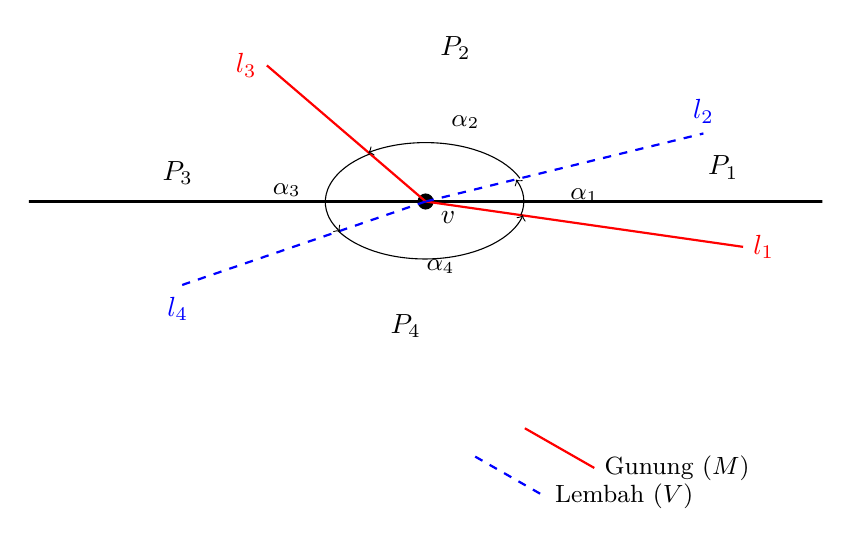
\begin{tikzpicture}[scale=1.8]
    % Kertas persegi
    \draw[thick, fill=gray!5] (-2,-2) rectangle (2,2);
    
    % Verteks pusat
    \filldraw[black] (0,0) circle (1.5pt) node[below right, xshift=2pt] {$v$};
    
    % Garis lipatan (creases) — 4 buah
    \draw[thick, red] (0,0) -- (2, 1.2) node[right] {$l_1$};
    \draw[thick, blue, dashed] (0,0) -- (0.8, 2) node[above] {$l_2$};
    \draw[thick, red] (0,0) -- (-2, 0.4) node[left] {$l_3$};
    \draw[thick, blue, dashed] (0,0) -- (-0.5, -2) node[below] {$l_4$};
    
    % Label panel
    \node at (1.2, 1.8) {$P_1$};
    \node at (-1.2, 1.5) {$P_2$};
    \node at (-1.5, -1.0) {$P_3$};
    \node at (1.0, -1.2) {$P_4$};
    
    % Sudut-sudut
    \draw[->] (0.6, 0.36) arc[start angle=31, end angle=68, radius=0.7];
    \node at (0.75, 0.85) {\small $\alpha_1$};
    
    \draw[->] (0.27, 0.68) arc[start angle=68, end angle=169, radius=0.73];
    \node at (-0.5, 0.9) {\small $\alpha_2$};
    
    \draw[->] (-0.7, 0.14) arc[start angle=169, end angle=256, radius=0.72];
    \node at (-0.8, -0.6) {\small $\alpha_3$};
    
    \draw[->] (-0.18, -0.7) arc[start angle=256, end angle=391, radius=0.72];
    \node at (0.65, -0.5) {\small $\alpha_4$};
    
    % Legenda
    \draw[thick, red] (2.5, -1.5) -- (3.2, -1.5) node[right, black] {\small Gunung ($M$)};
    \draw[thick, blue, dashed] (2.5, -2.0) -- (3.2, -2.0) node[right, black] {\small Lembah ($V$)};
  \end{tikzpicture}
  \caption{Pola lipatan (\textit{crease pattern}) dengan satu verteks interior $v$ berderajat empat. Garis merah solid merepresentasikan lipatan gunung ($M$) dan garis biru putus-putus merepresentasikan lipatan lembah ($V$).}
  \label{fig:crease_pattern}
\end{figure}

Pola lipatan pada sebuah verteks dikatakan dapat dilipat secara datar (\textit{flat-foldable}) jika panel-panel di sekitar verteks tersebut dapat dilipat hingga berhimpit pada satu bidang datar tanpa merobek kertas.

\subsection{Teorema Pelipatan Datar}
Dua teorema fundamental yang mengatur keseimbangan sudut dan garis lipatan pada satu titik verteks adalah Teorema Kawasaki dan Teorema Maekawa.
\begin{teorema}[Teorema Kawasaki]
  Misalkan $v$ adalah verteks tunggal di bagian dalam kertas dengan garis-garis lipatan yang bertemu di $v$ membentuk sudut-sudut $\alpha_1, \alpha_2, \ldots, \alpha_{2n}$ yang diurutkan secara sirkular. Pola lipatan di sekitar $v$ dapat dilipat datar (\textit{flat-foldable}) jika dan hanya jika jumlah sudut bolak-baliknya saling sama, yaitu:
  \[
    \alpha_1 + \alpha_3 + \ldots + \alpha_{2n-1} = \alpha_2 + \alpha_4 + \ldots + \alpha_{2n} = 180^\circ.
  \]
\end{teorema}

\begin{contoh}
  Tinjau verteks $v$ pada \ref{fig:crease_pattern} dengan empat garis lipatan yang membentuk sudut-sudut $\alpha_1 = 60^\circ$, $\alpha_2 = 120^\circ$, $\alpha_3 = 120^\circ$, $\alpha_4 = 60^\circ$ secara sirkular. Verifikasi Teorema Kawasaki:
  \[
    \alpha_1 + \alpha_3 = 60^\circ + 120^\circ = 180^\circ, \quad \alpha_2 + \alpha_4 = 120^\circ + 60^\circ = 180^\circ.
  \]
  Karena kedua jumlahan bolak-balik sama-sama bernilai $180^\circ$, maka verteks $v$ memenuhi syarat Kawasaki dan dapat dilipat datar.
\end{contoh}

Setiap garis lipatan pada pola pelipatan diberi penugasan kelengkungan berupa Gunung ($M$, \textit{Mountain}) atau Lembah ($V$, \textit{Valley}).
\begin{teorema}[Teorema Maekawa]
  Misalkan $M$ adalah banyaknya jumlah garis gunung dan $V$ adalah banyaknya jumlah garis lembah yang bertemu pada satu verteks interior di kertas. Jika verteks tersebut dapat dilipat secara datar (\textit{flat-foldable}), maka selisih antara jumlah lipatan gunung dan lembah adalah $2$ atau $-2$. Secara matematis ditulis sebagai:
  \[
    M - V = \pm 2.
  \]
\end{teorema}

\begin{contoh}
  Pada \ref{fig:crease_pattern}, garis lipatan $l_1$ dan $l_3$ bertipe gunung ($M$), sedangkan $l_2$ dan $l_4$ bertipe lembah ($V$). Maka $M = 2$ dan $V = 2$, sehingga $M - V = 0$. Penugasan tersebut \textbf{tidak} memenuhi Teorema Maekawa, karena $M - V \ne \pm 2$. Agar memenuhi, misalnya diubah menjadi $l_1, l_2, l_3$ bertipe gunung dan $l_4$ bertipe lembah, sehingga $M = 3$, $V = 1$, dan $M - V = 2$. Dengan demikian syarat Maekawa terpenuhi.
\end{contoh}

Berdasarkan Teorema Maekawa, jumlah derajat (\textit{degree}) atau banyaknya total garis lipatan pada setiap interior verteks pada pelipatan datar (\textit{flat folding}) pasti bernilai genap. Hal ini ditunjukkan oleh persamaan $M + V = (V \pm 2) + V = 2V \pm 2 \equiv 0 \pmod 2$.

\subsection{Matriks Ketetanggaan pada Graf Lipatan}
Karena pola lipatan pada dasarnya adalah graf planar, interaksi antar verteks dan panel dapat direpresentasikan secara aljabar linier menggunakan matriks ketetanggaan (\textit{adjacency matrix}).
\begin{definisi}
  Misalkan $G = (V, E)$ adalah graf planar lipatan dengan $n$ daerah panel. Matriks ketetanggaan $A$ berukuran $n \times n$ didefinisikan sebagai:
  \[
    A_{ij} = 
    \begin{cases}
      1, & \text{jika panel } i \text{ dan } j \text{ saling terhubung oleh satu garis lipatan}, \\
      0, & \text{lainnya}.
    \end{cases}
  \]
\end{definisi}

\begin{contoh}
  Dari pola lipatan pada \ref{fig:crease_pattern} terdapat empat panel $P_1, P_2, P_3, P_4$ yang dipisahkan oleh empat garis lipatan. Panel $P_1$ berbatasan dengan $P_2$ (melalui $l_2$) dan $P_4$ (melalui $l_1$). Panel $P_2$ berbatasan dengan $P_3$ (melalui $l_3$). Panel $P_3$ berbatasan dengan $P_4$ (melalui $l_4$). Matriks ketetanggaannya adalah:
  \[
    A = \begin{pmatrix}
      0 & 1 & 0 & 1 \\
      1 & 0 & 1 & 0 \\
      0 & 1 & 0 & 1 \\
      1 & 0 & 1 & 0
    \end{pmatrix}.
  \]
  Matriks ini simetris karena graf lipatan bersifat tak berarah. Entri $A_{12} = A_{21} = 1$ menunjukkan bahwa panel $P_1$ dan $P_2$ terhubung oleh garis lipatan $l_2$.
\end{contoh}

\begin{figure}[H]
  \centering
  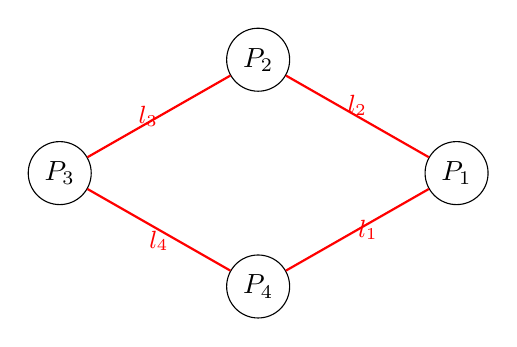
\begin{tikzpicture}[scale=1.2, every node/.style={circle, draw, minimum size=0.8cm, inner sep=0pt}]
    % Nodes (panel)
    \node (P1) at (1.5, 1.5) {$P_1$};
    \node (P2) at (-1.5, 1.5) {$P_2$};
    \node (P3) at (-1.5, -1.5) {$P_3$};
    \node (P4) at (1.5, -1.5) {$P_4$};
    
    % Edges (garis lipatan)
    \draw[thick, red] (P1) -- (P2) node[midway, above, draw=none, rectangle, minimum size=0pt] {\small $l_2$};
    \draw[thick, red] (P2) -- (P3) node[midway, left, draw=none, rectangle, minimum size=0pt] {\small $l_3$};
    \draw[thick, red] (P3) -- (P4) node[midway, below, draw=none, rectangle, minimum size=0pt] {\small $l_4$};
    \draw[thick, red] (P4) -- (P1) node[midway, right, draw=none, rectangle, minimum size=0pt] {\small $l_1$};
  \end{tikzpicture}
  \caption{Graf ketetanggaan dari pola lipatan pada \ref{fig:crease_pattern}. Setiap simpul merepresentasikan sebuah panel, dan setiap sisi merepresentasikan garis lipatan yang membatasi dua panel bertetanggaan.}
  \label{fig:adjacency_graph}
\end{figure}

Representasi matriks ini amat esensial karena di dalam komputasi pelipatan, pencarian urutan jalur transformasi spasial antar-panel diselesaikan dengan melacak elemen matriks non-nol yang menunjukkan batas ketetanggaan atau konektivitas mekanis engsel \parencite{ku2014realization}.

\section{Rigid Origami}
Dalam kinematika pelipatan kaku (\textit{rigid folding}), kertas direpresentasikan sebagai kumpulan panel polihedral (bidang datar) yang terhubung oleh engsel lurus berupa garis lipatan. Panel-panel ini dianggap sebagai benda tegar (\textit{rigid body}) yang tidak dapat ditekuk secara kontinu, melainkan hanya berputar secara kaku pada sumbu engsel lipatannya. Orientasi masing-masing panel dipetakan menggunakan transformasi spasial dalam ruang Euclidean $\R^3$.

\subsection{Transformasi Affine}
\begin{definisi}
  Suatu transformasi Affine pada ruang vektor $\R^n$ adalah suatu fungsi $f: \R^n \to \R^n$ yang dapat dinyatakan dalam bentuk
  \[
    f(\mathbf{x}) = A\mathbf{x} + \mathbf{b}
  \]
  di mana $A$ adalah pemetaan linear (berupa matriks berukuran $n \times n$) dan $\mathbf{b} \in \R^n$ adalah vektor translasi.
\end{definisi}

\begin{contoh}
  Misalkan transformasi Affine pada $\R^2$ didefinisikan oleh
  \[
    f(\mathbf{x}) = \begin{pmatrix} 0 & -1 \\ 1 & 0 \end{pmatrix} \mathbf{x} + \begin{pmatrix} 3 \\ 1 \end{pmatrix}.
  \]
  Jika $\mathbf{x} = (2, 5)^T$, maka
  \[
    f\!\begin{pmatrix} 2 \\ 5 \end{pmatrix} = \begin{pmatrix} 0 & -1 \\ 1 & 0 \end{pmatrix} \begin{pmatrix} 2 \\ 5 \end{pmatrix} + \begin{pmatrix} 3 \\ 1 \end{pmatrix} = \begin{pmatrix} -5 \\ 2 \end{pmatrix} + \begin{pmatrix} 3 \\ 1 \end{pmatrix} = \begin{pmatrix} -2 \\ 3 \end{pmatrix}.
  \]
  Transformasi ini memutar titik sejauh $90^\circ$ berlawanan arah jarum jam lalu menggesernya sebesar vektor $(3, 1)^T$.
\end{contoh}

Dalam pemodelan origami lipatan kaku, titik asal (origin) diletakkan tepat pada engsel, sehingga vektor translasi $\mathbf{b} = \mathbf{0}$, menjadikan transformasinya murni didominasi oleh operasi rotasi spasial.

\subsection{Grup Ortogonal Khusus $SO(3)$}
Pemetaan linear rotasi di ruang $\R^3$ dilakukan oleh anggota dari Grup Ortogonal Khusus (Special Orthogonal Group).
\begin{definisi}
  Grup ortogonal khusus derajat 3, dinotasikan dengan $SO(3)$, adalah grup perkalian matriks rotasi berukuran $3 \times 3$ berisikan elemen bilangan riil. Himpunan ini didefinisikan sebagai:
  \[
    SO(3) = \{ R \in \R^{3 \times 3} \mid R^T R = I_3, \det(R) = 1 \}
  \]
\end{definisi}

\begin{contoh}
  Jika sebuah engsel (garis lipatan) berada di sumbu-$x$, rotasi sebuah panel dengan sudut $\theta$ di sekitar sumbu-$x$ dihitung dengan perkalian matriks rotasi $R_x(\theta) \in SO(3)$:
  \[
    R_x(\theta) =
    \begin{pmatrix}
      1 & 0          & 0           \\
      0 & \cos\theta & -\sin\theta \\
      0 & \sin\theta & \cos\theta
    \end{pmatrix}
  \]
  Untuk sudut lipatan $\theta = 90^\circ$, diperoleh:
  \[
    R_x(90^\circ) =
    \begin{pmatrix}
      1 & 0 & 0  \\
      0 & 0 & -1 \\
      0 & 1 & 0
    \end{pmatrix}.
  \]
  Dapat diverifikasi bahwa $R_x(90^\circ)^T R_x(90^\circ) = I_3$ dan $\det(R_x(90^\circ)) = 1$.
\end{contoh}

\begin{figure}[H]
  \centering
  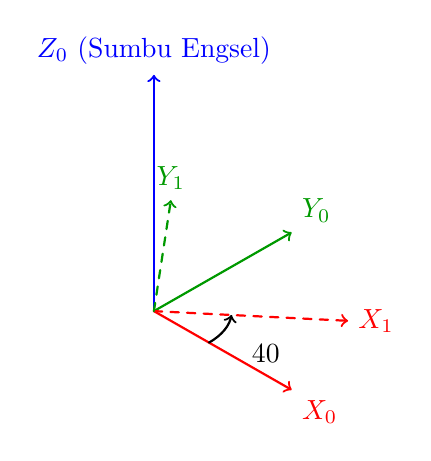
\begin{tikzpicture}[scale=2.5, line join=round, line cap=round]
    % Konfigurasi proyeksi 3D isometrik
    \tikzset{
      x={(0.7cm, -0.4cm)},
      y={(0.7cm, 0.4cm)},
      z={(0cm, 1cm)}
    }
    
    \coordinate (O) at (0,0,0);
    
    % Sumbu original (Frame 0)
    \draw[->, thick, red] (O) -- (1,0,0) node[below right] {$X_0$};
    \draw[->, thick, green!60!black] (O) -- (0,1,0) node[above right] {$Y_0$};
    \draw[->, thick, blue] (O) -- (0,0,1.2) node[above] {$Z_0$ (Sumbu Engsel)};
    
    % Sumbu rotasi (Frame 1) dirotasi sebesar theta
    \def\theta{40}
    \coordinate (X1) at ({cos(\theta)}, {sin(\theta)}, 0);
    \coordinate (Y1) at ({-sin(\theta)}, {cos(\theta)}, 0);
    
    \draw[->, thick, red, dashed] (O) -- (X1) node[right] {$X_1$};
    \draw[->, thick, green!60!black, dashed] (O) -- (Y1) node[above] {$Y_1$};
    
    % Arc sudut rotasi theta menggunakan segmen garis
    \draw[->, thick] (0.4, 0, 0) 
      \foreach \t in {5,10,...,35} {
        -- ({0.4*cos(\t)}, {0.4*sin(\t)}, 0)
      }
      -- ({0.4*cos(\theta)}, {0.4*sin(\theta)}, 0);
    
    \node[anchor=north west] at ({0.5*cos(\theta/2)}, {0.5*sin(\theta/2)}, 0) {$\theta$};
  \end{tikzpicture}
  \caption{Representasi vektor pada transformasi rotasi $SO(3)$ di seputar engsel origami. Kerangka awal $(X_0, Y_0)$ diputar sebesar sudut $\theta$ menjadi $(X_1, Y_1)$ terhadap sumbu engsel $Z_0$.}
  \label{fig:kinematics}
\end{figure}

Pergerakan dari panel pertama hingga panel terakhir yang mengitari satu verteks direpresentasikan oleh rantai perkalian sekuensial dari matriks-matriks $SO(3)$. Syarat \textit{loop closure} mengharuskan rantai perkalian ini kembali menjadi matriks identitas $I_3$. Operasi fungsi trigonometri berantai ini memicu latensi dan kompleksitas yang tinggi.

\subsection{Syarat Penutup Lengkung}
Transformasi spasial rotasi antar panel pada satu pola lipatan verteks tunggal (\textit{single vertex}) tidak terjadi secara independen. Terdapat sebuah batasan mekanis fisik bawaan yang mengharuskan bidang kertas tetap terhubung utuh mengitari verteks tanpa terjadi kerobekan.

\begin{teorema}[\textit{Loop Closure}]
  Misalkan suatu verteks tunggal dikelilingi secara sirkular oleh $k$ buah garis lipatan. Biarkan $R_1, R_2, \ldots, R_k \in SO(3)$ merepresentasikan matriks rotasi berantai yang melintasi setiap garis lipatan secara sekuensial. Agar kertas tetap bersambung, hasil komputasi perkalian dari serangkaian transformasi matriks tersebut wajib kembali ke orientasi awal mula, alias bernilai matriks identitas spasial:
  \[
    \prod_{i=1}^{k} R_i = R_1 R_2 \ldots R_k = I_3
  \]
\end{teorema}

\begin{contoh}
  Tinjau verteks dengan empat garis lipatan ($k = 4$) yang seluruhnya sejajar sumbu-$z$, dengan sudut-sudut lipatan $\theta_1 = 90^\circ$, $\theta_2 = 90^\circ$, $\theta_3 = 90^\circ$, $\theta_4 = 90^\circ$. Setiap rotasi parsial adalah:
  \[
    R_z(90^\circ) = \begin{pmatrix} 0 & -1 & 0 \\ 1 & 0 & 0 \\ 0 & 0 & 1 \end{pmatrix}.
  \]
  Maka rantai rotasi keseluruhan menghasilkan:
  \[
    R_z(90^\circ)^4 = R_z(360^\circ) = I_3.
  \]
  Syarat \textit{loop closure} terpenuhi karena empat rotasi $90^\circ$ berturut-turut pada sumbu yang sama menghasilkan rotasi penuh $360^\circ$, yaitu kembali ke orientasi awal.
\end{contoh}

Kondisi di atas dinamakan sebagai syarat \textit{Loop Closure Constraint}. Karena setiap matriks ortogonal $R_i$ memuat argumen fungsi sinus dan kosinus dari masing-masing sudut tekuk lipat (\textit{dihedral angle}), maka penyelesaian numeriknya memerlukan algoritma komputasi untuk menyelesaikan sistem persamaan trigonometri non-linear dengan orde komputasi tinggi. Studi literatur terbaru mengenai mekanisme infinitesimal tingkat kedua pada \textit{rigid origami} menunjukkan bahwa fenomena bifurkasi struktur spasial di sekitar kondisi ini menjadi subjek krusial dalam pergerakan dinamisnya \parencite{hayakawa2023analytical, hayakawa2024rigid}.

\subsection{Parametrisasi Rotasi $SO(3)$ melalui Sudut Euler dan Quaternion}
Analisis pergerakan kontinu di atas memanifestasikan kebutuhan parametrisasi matriks rotasi $R \in SO(3)$ yang presisi. Pendekatan analitik konvensional sering memecah $R$ menggunakan sudut Euler, di mana rotasi spasial didekomposisi atas rotasi parsial mengelilingi tiga sumbu koordinat utama ($X, Y, Z$).

Kelemahan utama pemanfaatan sudut Euler pada pelipatan origami terletak pada fenomena \textit{gimbal lock}, yaitu di mana dua sumbu rotasi menjadi sejajar, mengakibatkan hilangnya satu derajat kebebasan komputasional. Oleh karenanya, formulasi matematika lanjut menggunakan bilangan kompleks empat dimensi bernama \textit{Quaternion} lebih diminati.
\begin{definisi}
  Suatu unit quaternion $\mathbf{q} = q_0 + q_1 \mathbf{i} + q_2 \mathbf{j} + q_3 \mathbf{k}$ dengan magnitudo $|\mathbf{q}| = 1$ secara kanonik berkorespondensi mutlak dengan suatu rotasi di $SO(3)$. Transformasi pada vektor $\mathbf{v} \in \R^3$ menggunakan unit quaternion ini dirumuskan lewat operasi perkalian Hamilton:
  \[
    \mathbf{v}' = \mathbf{q} \mathbf{v} \mathbf{q}^{-1}
  \]
\end{definisi}

\begin{contoh}
  Rotasi sebesar $\theta = 90^\circ$ terhadap sumbu-$z$ (vektor satuan $\hat{\mathbf{u}} = (0,0,1)$) direpresentasikan oleh unit quaternion:
  \[
    \mathbf{q} = \cos\frac{90^\circ}{2} + \sin\frac{90^\circ}{2}\,(0\mathbf{i} + 0\mathbf{j} + 1\mathbf{k}) = \frac{\sqrt{2}}{2} + \frac{\sqrt{2}}{2}\mathbf{k}.
  \]
  Untuk memutar vektor $\mathbf{v} = (1, 0, 0)$ (yang diimbed menjadi quaternion murni $\mathbf{v} = 0 + 1\mathbf{i} + 0\mathbf{j} + 0\mathbf{k}$), dihitung:
  \[
    \mathbf{v}' = \mathbf{q}\mathbf{v}\mathbf{q}^{-1} = \left(\tfrac{\sqrt{2}}{2} + \tfrac{\sqrt{2}}{2}\mathbf{k}\right)(1\mathbf{i})\left(\tfrac{\sqrt{2}}{2} - \tfrac{\sqrt{2}}{2}\mathbf{k}\right) = 0 + 0\mathbf{i} + 1\mathbf{j} + 0\mathbf{k}.
  \]
  Dengan demikian, vektor $(1,0,0)$ diputar menjadi $(0,1,0)$, sesuai rotasi $90^\circ$ berlawanan arah jarum jam terhadap sumbu-$z$.
\end{contoh}

Perkalian komutatif quaternion secara dramatis menghindari limitasi \textit{gimbal lock} dan menyederhanakan perhitungan sekuensial yang terjadi berulang-ulang di setiap engsel. Namun, hal ini tidak mengeliminasi sifat non-linear bawaannya.

\subsection{Model Kinematika Denavit-Hartenberg}
Dengan menjadikan setiap panel origami sebagai lengan tegar dan engselnya sebagai sendi putar murni (\textit{revolute joint}), model kinematika origami secara ekuivalen sepadan dengan struktur rantai robotika (\textit{robotic chain}). 
\begin{definisi}
  Parameter Denavit-Hartenberg (D-H) mendeskripsikan keterikatan ruang antar dua pasang engsel yang berurutan dalam kerangka spasial melalui konvensi empat matriks parameter absolut:
  \[
    A_i = \text{Rot}_z(\theta_i) \text{Trans}_z(d_i) \text{Trans}_x(a_i) \text{Rot}_x(\alpha_i)
  \]
  di mana $\theta_i$ merupakan sudut lipat engsel origami, dan $\alpha_i$ adalah sudut sektor panel.
\end{definisi}

\begin{contoh}
  Pada origami satu verteks dengan empat garis lipatan, engsel pertama memiliki parameter D-H: sudut lipatan $\theta_1 = 90^\circ$, offset $d_1 = 0$ (karena engsel origami bersifat planar), panjang tautan $a_1 = 0$ (engsel bertemu di satu titik), dan sudut sektor $\alpha_1 = 60^\circ$ (sudut panel antara engsel pertama dan kedua). Matriks transformasinya adalah:
  \[
    A_1 = R_z(90^\circ) \cdot I \cdot I \cdot R_x(60^\circ) = \begin{pmatrix} 0 & -1 & 0 \\ 1 & 0 & 0 \\ 0 & 0 & 1 \end{pmatrix} \begin{pmatrix} 1 & 0 & 0 \\ 0 & \frac{1}{2} & -\frac{\sqrt{3}}{2} \\ 0 & \frac{\sqrt{3}}{2} & \frac{1}{2} \end{pmatrix}.
  \]
\end{contoh}

Formulasi mekanika analitik D-H ini memperkuat abstraksi penyelesaian \textit{loop closure} ke tingkat di mana perkalian majemuk dari seluruh parameter ekuivalen dengan pembentukan sebuah lengkung kurva non-trivial berderajat jamak di ruang dimensi tinggi.

\section{Geometri Tropikal}
Sebagai alternatif, geometri tropikal akan digunakan untuk menyederhanakan perhitungan non-linear trigonometris yang rumit pada ruang kontinu menjadi perhitungan logis fungsi linear secara lokal \parencite{mikhalkin2006tropical}.

\subsection{Aljabar Min-Plus}
Geometri tropikal dibangun di atas landasan struktur semiring tropikal, dengan salah satu contoh utamanya adalah aljabar min-plus.
\begin{definisi}
  Aljabar min-plus adalah himpunan bilangan real yang diperluas $\R_{\min} = \R \cup \{\infty\}$ yang dilengkapi dengan dua operasi biner utama, yaitu operasi penjumlahan tropikal ($\oplus$) dan perkalian tropikal ($\otimes$):
  \begin{align*}
    a \oplus b  & = \min\{a, b\}, \quad \forall a, b \in \R_{\min} \\
    a \otimes b & = a + b, \quad \forall a, b \in \R_{\min}
  \end{align*}
  Elemen identitas untuk operasi $\oplus$ adalah $\infty$, dan elemen identitas untuk operasi $\otimes$ adalah $0$.
\end{definisi}

\begin{contoh}
  Evaluasi operasi aritmetika pada semiring aljabar tropikal min-plus untuk bilangan skalar menghasilkan perhitungan berikut:
  \begin{align*}
    5 \oplus 7  & = \min(5, 7) = 5 \\
    5 \otimes 7 & = 5 + 7 = 12
  \end{align*}
\end{contoh}

Sistem ini dinamakan semiring karena memenuhi sifat-sifat dasar gelanggang (ring) seperti komutatif dan distributif, namun tidak memiliki invers terhadap operasi penjumlahan $\oplus$.

\begin{contoh}
  Operasi matriks juga dapat didefinisikan pada aljabar min-plus. Misalkan
  \[
    A = \begin{pmatrix} 1 & 3 \\ 2 & 0 \end{pmatrix}, \quad B = \begin{pmatrix} 4 & 1 \\ \infty & 2 \end{pmatrix}.
  \]
  Perkalian matriks tropikal $C = A \otimes B$ dihitung sebagai:
  \[
    C_{ij} = \bigoplus_{k} (A_{ik} \otimes B_{kj}) = \min_k (A_{ik} + B_{kj}).
  \]
  Maka:
  \begin{align*}
    C_{11} &= \min(1+4,\; 3+\infty) = \min(5, \infty) = 5, \\
    C_{12} &= \min(1+1,\; 3+2) = \min(2, 5) = 2, \\
    C_{21} &= \min(2+4,\; 0+\infty) = \min(6, \infty) = 6, \\
    C_{22} &= \min(2+1,\; 0+2) = \min(3, 2) = 2.
  \end{align*}
  Jadi $C = \begin{pmatrix} 5 & 2 \\ 6 & 2 \end{pmatrix}$.
\end{contoh}

\subsection{Fungsi \textit{Piecewise-Affine} Tropikal}
Dekuantisasi fungsi aljabar biasa menuju ranah semiring min-plus akan mereduksi kurva fungsi derajat tinggi menjadi sebuah kompleks fungsi linear sepotong-sepotong (\textit{piecewise-affine}).

\begin{definisi}
  Polinomial tropikal dalam $n$ variabel $x_1, \ldots, x_n$ adalah sebuah pemetaan fungsi $p: \R^n \to \R$ yang didefinisikan secara struktur min-plus sebagai:
  \[
    p(x_1, \ldots, x_n) = \bigoplus_{\mathbf{v} \in V} c_{\mathbf{v}} \otimes x_1^{\otimes v_1} \otimes \ldots \otimes x_n^{\otimes v_n}
  \]
  di mana $V \subset \Z_{\ge 0}^n$ adalah sebuah himpunan berhingga, dan $c_{\mathbf{v}} \in \R_{\min}$. Jika dijabarkan ke aljabar numerik standar, polinomial tropikal mendefinisikan fungsi konveks minimum yang bersifat \textit{piecewise-affine}:
  \[
    p(x) = \min_{\mathbf{v} \in V} \left( c_{\mathbf{v}} + \sum_{i=1}^n v_i x_i \right)
  \]
\end{definisi}

\begin{contoh}
  Tinjau polinomial tropikal dalam satu variabel:
  \[
    p(x) = (2 \otimes x^{\otimes 2}) \oplus (1 \otimes x) \oplus 3 = \min(2 + 2x,\; 1 + x,\; 3).
  \]
  Fungsi ini terdiri dari tiga segmen linear. Untuk menentukan akar tropikal (titik di mana minimum dicapai dua kali), diselesaikan:
  \begin{itemize}
    \item $2 + 2x = 1 + x \implies x = -1$. Cek: $p(-1) = \min(0, 0, 3) = 0$. \checkmark
    \item $1 + x = 3 \implies x = 2$. Cek: $p(2) = \min(6, 3, 3) = 3$. \checkmark
  \end{itemize}
  Polinomial tropikal ini memiliki dua akar, yaitu $x = -1$ dan $x = 2$, yang merupakan titik-titik patahan (\textit{breakpoints}) pada grafik fungsi \textit{piecewise-affine}.
\end{contoh}

\begin{figure}[H]
  \centering
  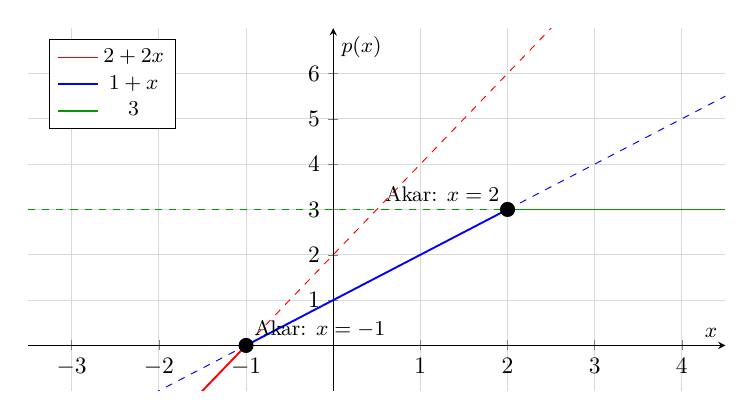
\begin{tikzpicture}[scale=0.85]
    \begin{axis}[
      axis lines=middle,
      xlabel={$x$},
      ylabel={$p(x)$},
      xmin=-3.5, xmax=4.5,
      ymin=-1, ymax=7,
      width=12cm, height=7cm,
      grid=major,
      grid style={gray!30},
      xtick={-3,-2,-1,0,1,2,3,4},
      ytick={0,1,2,3,4,5,6},
      legend pos=north west,
      legend style={font=\small},
      every axis label/.style={font=\small},
    ]
      % Segmen 1: 2 + 2x (dominan untuk x < -1)
      \addplot[domain=-3.5:-1, thick, red] {2 + 2*x};
      \addlegendentry{$2+2x$}
      
      % Segmen 2: 1 + x (dominan untuk -1 < x < 2)
      \addplot[domain=-1:2, thick, blue] {1 + x};
      \addlegendentry{$1+x$}
      
      % Segmen 3: 3 (dominan untuk x > 2)
      \addplot[domain=2:4.5, thick, green!60!black] {3};
      \addlegendentry{$3$}
      
      % Garis-garis non-dominan (putus-putus)
      \addplot[domain=-1:4.5, thin, red, dashed] {2 + 2*x};
      \addplot[domain=-3.5:-1, thin, blue, dashed] {1 + x};
      \addplot[domain=2:4.5, thin, blue, dashed] {1 + x};
      \addplot[domain=-3.5:2, thin, green!60!black, dashed] {3};
      
      % Titik-titik patahan (akar tropikal)
      \addplot[only marks, mark=*, mark size=3pt, black] coordinates {(-1, 0) (2, 3)};
      \node[above right] at (axis cs:-1, 0) {\small Akar: $x=-1$};
      \node[above left] at (axis cs:2, 3) {\small Akar: $x=2$};
    \end{axis}
  \end{tikzpicture}
  \caption{Grafik polinomial tropikal $p(x) = \min(2+2x,\; 1+x,\; 3)$. Garis tebal menunjukkan segmen minimum yang aktif (fungsi \textit{piecewise-affine}). Titik-titik patahan adalah akar tropikal.}
  \label{fig:tropical_polynomial}
\end{figure}

\subsection{Permukaan Tropikal dan Syarat Keseimbangan}
Polinomial fungsi nilai ekstrem minimum tropikal membentuk suatu topologi geometri spasial polihedral. Di dalam lanskap fungsi berdimensi jamak, sebuah kompleks permukaan di mana fungsi ini bersifat nondiferensiabel---yaitu daerah perpotongan di mana nilai minimum dicapai secara identik dan simultan oleh sedikitnya dua term affine---disebut sebagai permukaan hiper tropikal (\textit{tropical hypersurfaces}) \parencite{maclagan2015tropical}.

\begin{definisi}
  Suatu \textit{tropical hypersurface} $V(p)$ dari sebuah persamaan polinomial tropikal $p(\mathbf{x}) = \min_{\mathbf{v} \in V} \left( c_{\mathbf{v}} + \langle \mathbf{v}, \mathbf{x} \rangle \right)$ didefinisikan sebagai himpunan titik vektor $\mathbf{x} \in \R^n$ di mana batas nilai ekstrem minimum pada polinomial tersebut dicapai oleh minimal dua suku (\textit{term}) affine yang berbeda. 
\end{definisi}

\begin{contoh}
  Tinjau polinomial tropikal dua variabel $p(x,y) = x \oplus y \oplus 0 = \min(x, y, 0)$. Himpunan $V(p)$ terdiri dari titik-titik $(x,y) \in \R^2$ di mana minimum dicapai setidaknya dua kali:
  \begin{itemize}
    \item $x = y \leq 0$: sinar dari titik asal ke arah $\langle 1, 1 \rangle$ (untuk nilai negatif),
    \item $x = 0 \leq y$: sinar dari titik asal ke arah $\langle 0, -1 \rangle$ (untuk $y$ negatif, $x = 0$),
    \item $y = 0 \leq x$: sinar dari titik asal ke arah $\langle -1, 0 \rangle$ (untuk $x$ negatif, $y = 0$).
  \end{itemize}
  Ketiga sinar ini bertemu di titik asal $(0,0)$, membentuk sebuah kurva tropikal yang disebut garis tropikal (\textit{tropical line}).
\end{contoh}

\begin{figure}[H]
  \centering
  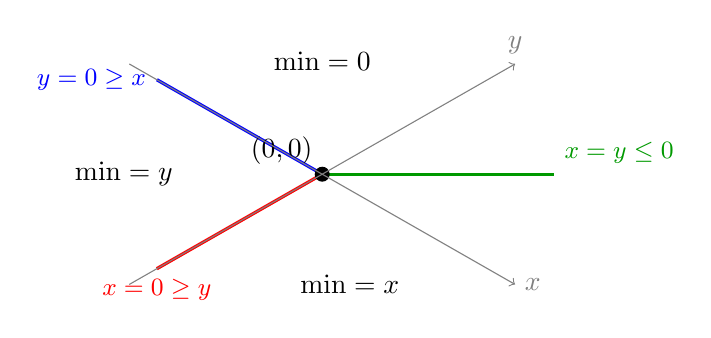
\begin{tikzpicture}[scale=1.0]
    % Sinar-sinar garis tropikal
    \draw[very thick, blue] (0,0) -- (-3, 0) node[left] {\small $y = 0 \geq x$};
    \draw[very thick, red] (0,0) -- (0, -3) node[below] {\small $x = 0 \geq y$};
    \draw[very thick, green!60!black] (0,0) -- (2.1, 2.1) node[above right] {\small $x = y \leq 0$};
    
    % Titik verteks
    \filldraw[black] (0,0) circle (2.5pt);
    \node[above left] at (0,0) {$(0,0)$};
    
    % Label daerah
    \node at (-1.8, -1.8) {$\min = y$};
    \node at (2.0, -1.5) {$\min = x$};
    \node at (-1.8, 1.8) {$\min = 0$};
    
    % Sumbu koordinat
    \draw[thin, gray, ->] (-3.5, 0) -- (3.5, 0) node[right] {$x$};
    \draw[thin, gray, ->] (0, -3.5) -- (0, 3.5) node[above] {$y$};
  \end{tikzpicture}
  \caption{Garis tropikal (\textit{tropical line}) $V(p)$ untuk $p(x,y) = \min(x, y, 0)$. Tiga sinar berbobot satu bertemu di verteks $(0,0)$.}
  \label{fig:tropical_line}
\end{figure}

Konsekuensi struktural yang lahir dari definisi tersebut adalah berlakunya hukum perimbangan pada tiap garis perpotongan.
\begin{teorema}[\textit{Balancing Condition}]
  Setiap titik persimpangan atau persambungan interior pada struktur \textit{tropical hypersurface} wajib memenuhi syarat kondisi perimbangan keseimbangan (\textit{balancing condition}). Untuk sebuah titik persimpangan verteks sebarang di dalam kerangka $V(p)$, suatu jumlahan berbobot (\textit{weighted sum}) dari serangkaian vektor arah (\textit{primitive integer vectors}) yang bertolak dari titik tersebut dan menyebar mengarah pada setiap sisi-sisi ketersambungan yang insiden dengannya, haruslah ekuivalen dan bernilai ekuilibrium nol:
  \[
    \sum_{j} w_j \cdot \mathbf{v}_j = \mathbf{0}
  \]
  di mana skalar $w_j \in \Z^+$ menyatakan bobot beban komputasi numerik (\textit{weight}) pada sisi lintasan ke-$j$.
\end{teorema}

\begin{contoh}
  Pada garis tropikal di \ref{fig:tropical_line}, ketiga sinar memiliki bobot $w_j = 1$ dan vektor arah primitif:
  \[
    \mathbf{v}_1 = \begin{pmatrix} -1 \\ 0 \end{pmatrix}, \quad \mathbf{v}_2 = \begin{pmatrix} 0 \\ -1 \end{pmatrix}, \quad \mathbf{v}_3 = \begin{pmatrix} 1 \\ 1 \end{pmatrix}.
  \]
  Syarat keseimbangan diverifikasi:
  \[
    1 \cdot \begin{pmatrix} -1 \\ 0 \end{pmatrix} + 1 \cdot \begin{pmatrix} 0 \\ -1 \end{pmatrix} + 1 \cdot \begin{pmatrix} 1 \\ 1 \end{pmatrix} = \begin{pmatrix} 0 \\ 0 \end{pmatrix}. \quad \checkmark
  \]
\end{contoh}

Pada pemodelan \textit{rigid folding} origami yang diusulkan, \textit{loop closure constraint} dari transformasi isometri rotasi engsel verteks kontinu akan diformulasikan ke dalam diskritisasi himpunan akar polinomial nilai-minimum tropikal menjadi \textit{tropical hypersurfaces}. Terdapat ekuivalensi yang kuat antara hukum perimbangan \textit{balancing condition} tropikal (di mana vektor-vektor yang bertolak dari simpangan berjumlah total nol) dengan Teorema Kawasaki dan Teorema Maekawa (penjumlahan dan perimbangan sudut lipatan gunung/lembah di titik pusat verteks interior). Oleh karenanya, kondisi struktural yang bersifat linear konveks ini bertindak secara sempurna menyulih peran non-linear konvensional dalam menjaga integritas jaring tata ruang pelipatan kertas secara utuh.

\subsection{Kurva Tropikal dan Poligon Newton}
Untuk dapat melakukan representasi visual terhadap interaksi suku-suku (terms) pada polinomial tropikal, parameter geometris konveks divisualisasikan dalam bentuk poligon batas.
\begin{definisi}
  Poligon Newton (\textit{Newton Polygon}), disimbolkan $\Delta(p)$, dari suatu fungsi polinomial tropikal dua variabel $p(x, y) = \bigoplus_{(i,j)} c_{i,j} \otimes x^{\otimes i} \otimes y^{\otimes j}$ adalah selubung cembung (\textit{convex hull}) dari seluruh kumpulan titik eksponen $(i,j)$ di dalam bidang dimensi-2 berkoordinat riil sedemikian sehingga koefisiennya bernilai terhingga ($c_{i,j} \ne \infty$).
\end{definisi}

\begin{contoh}
  Tinjau polinomial tropikal derajat 2:
  \[
    p(x,y) = x^{\otimes 2} \oplus (x \otimes y) \oplus y^{\otimes 2} \oplus x \oplus y \oplus 0 = \min(2x, x+y, 2y, x, y, 0).
  \]
  Himpunan eksponen yang muncul adalah $S = \{(2,0), (1,1), (0,2), (1,0), (0,1), (0,0)\}$, dan semua koefisien $c_{i,j} = 0$. Poligon Newton $\Delta(p)$ adalah selubung cembung dari $S$, yaitu segitiga dengan verteks $(0,0)$, $(2,0)$, dan $(0,2)$. Segitiga ini disebut segitiga berderajat 2 ($T_2$).
\end{contoh}

\begin{figure}[H]
  \centering
  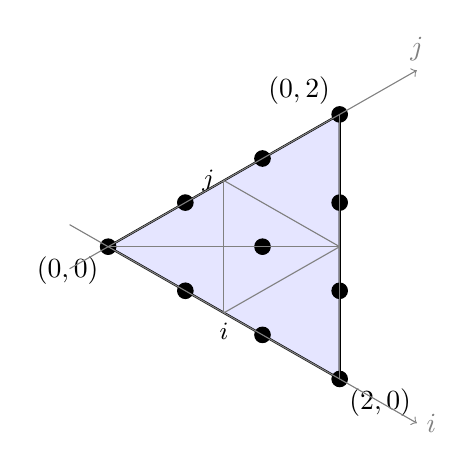
\begin{tikzpicture}[scale=1.4]
    % Poligon Newton
    \draw[thick, fill=blue!10] (0,0) -- (3,0) -- (0,3) -- cycle;
    
    % Titik-titik kisi
    \foreach \i in {0,...,3} {
      \foreach \j in {0,...,3} {
        \pgfmathparse{int(\i+\j)}
        \ifnum\pgfmathresult<4
          \filldraw[black] (\i, \j) circle (2pt);
        \fi
      }
    }
    
    % Label verteks
    \node[below left] at (0,0) {$(0,0)$};
    \node[below right] at (3,0) {$(2,0)$};
    \node[above left] at (0,3) {$(0,2)$};
    
    % Label tengah
    \node[below] at (1.5, 0) {\small $i$};
    \node[left] at (0, 1.5) {\small $j$};
    
    % Subdivisi interior (contoh)
    \draw[thin, gray] (0,0) -- (1.5, 1.5);
    \draw[thin, gray] (3,0) -- (0, 3);
    \draw[thin, gray] (1.5, 0) -- (0, 1.5);
    \draw[thin, gray] (1.5, 0) -- (1.5, 1.5);
    \draw[thin, gray] (0, 1.5) -- (1.5, 1.5);
    
    % Sumbu
    \draw[thin, gray, ->] (-0.5, 0) -- (4, 0) node[right] {$i$};
    \draw[thin, gray, ->] (0, -0.5) -- (0, 4) node[above] {$j$};
  \end{tikzpicture}
  \caption{Poligon Newton $\Delta(p) = T_2$ (segitiga berderajat 2) beserta titik-titik kisi interior dan subdivisi yang diinduksi oleh koefisien polinomial tropikal.}
  \label{fig:newton_polygon_new}
\end{figure}

Triangulasi dari Poligon Newton berkorespondensi langsung secara dual dengan konfigurasi kurva tropikal pada ruang nilai nyata. Garis-garis yang membentuk tulang punggung kurva tropikal senantiasa ortogonal secara topologis terhadap segmen garis triangulasi poligon Newton.

Sifat korelasi dualitas struktur kombinatorik ini memberikan fleksibilitas komputasi yang menjanjikan, di mana manipulasi topologis fungsi polinomial dapat diproyeksikan langsung terhadap titik-titik diskret pada ruang eksponennya yang linear tanpa perlu menggunakan metode komputasi matriks \textit{floating point} non-linear rumit layaknya pada struktur spasial trigonometri $SO(3)$.

\subsection{Teorema Kapranov}
Alasan mendasar mengapa pergerakan isometri origami dapat dialihbahasakan ke semiring tropikal adalah landasan fundamental geometri tropikal yang dikenal sebagai Teorema Kapranov.
\begin{teorema}[Teorema Kapranov]
  Untuk sebarang himpunan bilangan riil pada polinomial atas ruang Puiseux (aljabar terstruktur metrik diskret), \textit{tropical hypersurface} $V(p)$ dari ideal polinomial $p$ sama halnya dengan penutupan dari ruang limit evaluasi nilai (valuation) atas persimpangan semua titik akar dari varietas aljabarnya secara klasik.
\end{teorema}

Keterikatan absolut ini membuktikan jaminan matematis secara pasti bahwa kalkulasi minimum polinomial tropikal pada matriks ketetanggaan origami, meskipun terlihat sangat diskret dan dipenuhi persamaan garis kaku (\textit{piecewise}), secara akurat tetap menyajikan bayangan presisi penuh atas gerakan membelok kontinu ruang spasial origami. Hal ini juga menjadi landasan pengukuran isometri menggunakan pemetaan metrik Abel-Jacobi, menjamin keabsahan jarak rotasional \parencite{foster2020metric}.